\documentclass{standalone}
\usepackage{tikz}
\usepackage{ctex,siunitx}
\usepackage{tkz-euclide}
\usepackage{amsmath}
\usetikzlibrary{patterns, calc}
\usetikzlibrary {decorations.pathmorphing, decorations.pathreplacing, decorations.shapes,}
\begin{document}
\small
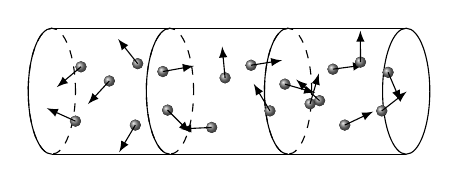
\begin{tikzpicture}[>=latex,scale=1.0]
  \draw(0,.8)--(4.5,.8);
  \draw(0,-.8)--(4.5,-.8);
  \draw[dashed](0,0)ellipse[x radius=.3, y radius=.8]; 
  \draw[dashed](1.5,0)ellipse[x radius=.3, y radius=.8]; 
  \draw[dashed](3,0)ellipse[x radius=.3, y radius=.8]; 
  \draw (4.5,0) ellipse[x radius=.3, y radius=.8]; 
  \draw(0,.8) arc [start angle = 90, end angle=270, x radius=.3, y radius=.8];
  \draw(1.5,.8) arc [start angle = 90, end angle=270, x radius=.3, y radius=.8];
  \draw(3.0,.8) arc [start angle = 90, end angle=270, x radius=.3, y radius=.8];
  \foreach \x/\y in { 0.30/-0.38,0.37/ 0.31,0.73/ 0.13,1.09/ 0.35,1.41/ 0.25,1.06/-0.43,1.47/-0.24,2.03/-0.46,2.20/ 0.17,2.53/ 0.33,2.96/ 0.09,2.77/-0.25,3.28/-0.16,3.40/-0.12,3.72/-0.43,4.19/-0.25,3.57/ 0.28,3.92/ 0.37,4.27/ 0.24 } 
    {
      \fill[ball color=gray ](\x,\y)circle(2pt);
      \draw[thin,->](\x,\y)--++(rand*360:0.4);
    }
\end{tikzpicture}
\end{document}